
\chapter{Lecture 5: Conditional probability}
At the time of writing (in december 2015), the Australian Bureau of Statistics reported that the median starting salary for bachelor degree graduates in all fields was \$52,500. However, the median starting salary for bachelor degree graduates in the field of mathematics was \$60,000. \\

\noindent Extra information (i.e., a ``\textbf{condition}''), can modify a probability. For example, if you engage in field of study $X$, then your chance of a higher salary is raised by a factor of $Y$. \label{condition} \\

\subsection{Example} \label{ex501}
Recall the two dice example \ref{example2.2.1} on page \pageref{example2.2.1}. The events we were interested in are
\begin{itemize}
\item $A = \set{\text{Outcomes where the total shown on two dice is 6}}$
\item $B = \set{\text{Outcomes where the total shown on two dice is 2}}$
\item $C = \set{\text{Outcomes where at least one of the dice shows a 1}}$
\end{itemize}
We found that
\[
P(A) = \frac{5}{36}, \qquad P(B) = \frac{1}{36}, \qquad P(C) = \frac{11}{36}
\]
\textbf{Question 1:} If we're given that event $A$ has happened (when we do our trial), then would we consider event $B$ to be more or less likely? \\
Answer: \textit{If A has happened, then the probability of B is zero.} \\
To understand this, just think about what the events themseves are. If $A$ has happened, then this means that the total shown on the two dice is exactly 6. Thus it is not possible for the dice to show a total of exactly 2, since we already know that the total is 6. Hence, the probability of $B$, given that $A$ occurred, is zero. \\

\noindent \textbf{Question 2:} If we're told that event $C$ has happened (in our trial), would we consider event $A$ to be more or less likely? \\
Answer: \textit{If $C$ has happened, then $A$ is more likely.} \\
To understand how the extra information about $C$ changes the probability of $A$, we again need to look at the events themselves. If $C$ has happened, then we can think of $C$ as being our new outcome space, because any outcome that is not in $C$ cannot occur. In example \ref{example2.2.1} we listed all the elements in $C$. They were
\[
C = \set{(1,1),(1,2),(1,3),(1,4),(1,5),(1,6),(2,1),(3,1),(4,1),(5,1),(6,1)}
\]
In only two of these outcomes do the dice add to a total of 6, they are $(1,5)$ and $(5,1).$ In other words, only two out of the 11 outcomes from $C$ are also elements of $A$. You should be getting familiar with assigning probabilities in situations where the outcomes are all equally likely. For a revision of how this is done see section \ref{sec222} on page \pageref{sec222}. In event $C$, all the outcomes are equally likely because the dice are fair. So, the new probability of $A$ (conditional on $C$), is given by the number of ways that $A$ can occur (2 ways in this case), divided by the size of the outcome space (11, the size of $C$, in this case). So the probability of $A$ given that $C$ has occurred is $2/11 \approx 0.18.$ This is indeed higher than the probability that we had for $A$ when there were no conditions (which was $5/36 \approx 0.13$). Note that the $\approx$ symbol means ``approximately equal to.'' We use this symbol because there are too many digits (after the decimal point) for us to completely accurately represent the full numbers in decimal form. \label{symbapprox} \\

\noindent \textbf{Question 3:} If we know that event $B$ has happened (in our trial), would we consider event $C$ to be more, or less, likely? \\
Answer: \textit{If $B$ has happened, then $C$ is more likely} \\
Again, we must look at the events themselves. If $B$ has happened, then the total shown on the two dice is exactly 2. This can only ever happen if both of the dice are showing 1. Hence, the event, $C$, that at least one of the dice shows 1, has now definitely happened. So the probability of $C$ is now equal to 1, i.e., $C$ is more likely.

\subsection{Conditional probability on a Venn diagram} \label{sec507}
During queston 2, in the previous example (example \ref{ex501}), it was mentioned that, if an event $C$ has happened, then we can think of $C$ as being our new outcome space. Really, this is what we mean when we say that ``$C$ has happened;'' we mean that now (i.e, for this trial) the only possible outcomes are those that lie within the event $C$. One way to visualise this is on a Venn diagram. Using the events $A,B,C$ from the previous example, if we have no condition (no event is claimed to have occurred) then the Venn diagram is
\begin{center}
	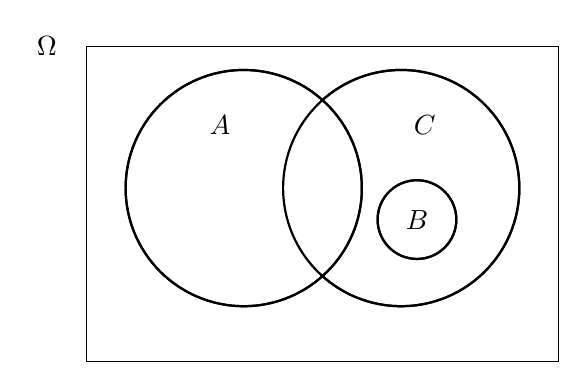
\begin{tikzpicture} [fill = white]
	\draw [fill = white] (-3,-2) -- (-3,2) -- (3,2) -- (3,-2) -- cycle;
	%\draw [fill = white] (-0.5,0.8) ellipse (1.6cm and 0.8cm);
	\draw [thick, fill = white] (1,0.2) circle (1.5);
	\draw [thick, fill = white] (-1,0.2) circle (1.5);
	\draw [thick, fill = white] (1.2,-0.2) circle (0.5);
	%\scope
	%\clip (0,-0.5) circle (1.3);
	%\fill (-1,0.4) circle (1.3);
	%\endscope
	\draw [thick] (1,0.2) circle (1.5);
	\draw [thick] (-1,0.2) circle (1.5);
	\draw [thick] (1.2,-0.2) circle (0.5);
	%\draw [thick] (1.4,0) circle (1.5);
	%\draw [thick] (-0.5,0.8) ellipse (1.6cm and 0.8cm);
	\draw (1.3,1) node {$C$};
	\draw (-3.5,2) node {$\Omega$};
	\draw (-1.3,1) node {$A$};
	\draw (1.2,-0.2) node {$B$};
	%\draw (0,0) node {$A \cap B$};
	\end{tikzpicture}
\end{center}
If, on the other hand, $C$ has occurred, then the new Venn diagram is obtained by excluding everything outside of $C$. Thus we obtain the following Venn diagram,
\begin{center}
	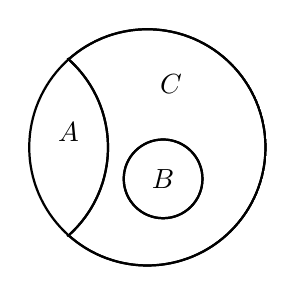
\begin{tikzpicture} [fill = white]
	\scope
	\clip (1,0.2) circle (1.52);
	%\draw [fill = white] (-0.5,0.8) ellipse (1.6cm and 0.8cm);
	\draw [thick, fill = white] (1,0.2) circle (1.5);
	\draw [thick, fill = white] (-1,0.2) circle (1.5);
	\draw [thick, fill = white] (1.2,-0.2) circle (0.5);
	%\scope
	%\clip (0,-0.5) circle (1.3);
	%\endscope
	\draw [thick] (1,0.2) circle (1.5);
	\draw [thick] (-1,0.2) circle (1.5);
	\draw [thick] (1.2,-0.2) circle (0.5);
	%\draw [thick] (1.4,0) circle (1.5);
	%\draw [thick] (-0.5,0.8) ellipse (1.6cm and 0.8cm);
	\draw (1.3,1) node {$C$};
	\draw (-3.5,2) node {$\Omega$};
	\draw (0,0.4) node {$A$};
	\draw (1.2,-0.2) node {$B$};
	\endscope
	%\draw (0,0) node {$A \cap B$};
	\end{tikzpicture}
\end{center}
We can see that $C$ now represents the entire outcome space. Notice that the only areas that are visible in the new Ven diagram are intersections of events with $C$ (i.e., $A \cap C$ and $B \cap C$). 

\subsection{Definition of conditional probability} \label{sec508}
Before expressing the formal definition of conditional probability we need some notation to represent conditional probabilities. To express the probability of an event $E$ given that another event $F$ has occurred we write \label{symbconditional} \label{conditional probability}
\bigskip

\hfil\fbox{
\begin{minipage}{0.13\columnwidth}{

\vskip 0.02cm
\begin{center}
$P(E \! \mid \! F)$
\end{center}
}
\end{minipage}}
\bigskip

\noindent We read this as, ``The probability of $E$ given that $F$ has occurred,'' or equivalently, ``the probability of $E$ conditional on $F$.'' \\

\noindent In order to find the probabiltiy of $E$ conditional on $F$, we need to use the formal definition of $P(E \! \mid \! F)$. The formal definition is
\bigskip

\hfil\fbox{
\begin{minipage}{0.3\columnwidth}{

\vskip 0.02cm
\begin{center}
$\displaystyle{P(E \! \mid \! F) = \frac{P(E \cap F)}{P(F)}}$
\end{center}
}
\end{minipage}}
\bigskip

\noindent We can check, for example, that this definition agrees with our result from question 2, in example \ref{ex501}, where we found $P(A \! \mid \! C)$. In question 2, we found all of the elements in $A$ that were in $C$, that is, we found $A \cap C$,
\[
A \cap C = \set{(1,5),(5,1)}
\]
Since $A \cap C$ has 2 elements and $|\Omega| = 36$, the (non-conditional) probability of $A \cap C$ is $2/36,$ i.e., $P(A \cap C) = 2/36.$ We also have from example \ref{ex501} that $P(C) = 11/36$. So, using the formal definition of conditional probability we have,
\[
P(A \mid C) = \frac{P(A \cap C)}{P(C)} = \frac{2/36}{11/36} = \frac{2}{36}\times\frac{36}{11} = \frac{2}{11}
\]
which is the same result that we obtained in question 2 using our own reasoning. \\

\noindent Note that the definition of conditional probability \textbf{does not make any sense if} $\boldsymbol{P(F) = 0}.$ The defintion requires us to divide by $P(F)$, so, if $P(F) = 0,$ then we would be required to divide by zero. Recall that if $P(F) = 0$, then $F$ occurring is impossible; intuitively, it does not make sense for us to ask, ``what is the probability of $E$ given that the impossible, $F$, has happened?''

\subsection{Example}
We will use the definition of conditional probability to check our results for question 1 and 2 from example \ref{ex501}. \\

\noindent In question 1 we wanted to find $P(B\! \mid \! A)$. Firstly, notice that $A$ and $B$ are disjoint, i.e.,~$B~\cap~A~=~\varnothing$. Hence $P(B \cap A) = 0$. So, using the definition of conditional probability,
\[
P(B \! \mid \! A) = \frac{P(B \cap A)}{P(A)} = \frac{0}{P(A)} = 0.
\]
This agrees with our result from question 1. \\

\noindent In question 3 we wanted to find $P(C \! \mid \! B)$. Firstly, notice that $B$ is fully contained within $C$ (see the venn diagrams in section \ref{sec507}). So, $P(C \cap B) = P(B)$. Hence, using the definition of conditional probability,
\[
P(C \! \mid \! B) = \frac{P(C \cap B)}{P(B)} = \frac{P(B)}{P(B)} = 1.
\]
This agrees with our result from question 3.

\subsection{The multiplication law} \label{multiplication law}
Not to be confused with the multiplication \textit{rule} from section \ref{secmult}; the multiplication law is really just a rearrangement of the formula in the definition of conditional probability. Concretely, suppose that we know $P(E \!\mid \! F)$ and $P(F)$ already, and we want to use these to find $P(E \cap F)$. Then, starting with the definition of conditional probability, and assuming $P(F) > 0$,
\[
P(E \! \mid \! F) = \frac{P(E \cap F)}{P(F)},
\]
we can multiply both sides by $P(F)$ to get \label{the multiplication law}
\bigskip

\hfil\fbox{
\begin{minipage}{0.6\columnwidth}{

\vskip 0.02cm
\begin{center}
$\displaystyle{P(E \! \mid \! F)P(F) = P(E \cap F), \hspace{0.5cm} \text{where} \; P(F) > 0.}$
\end{center}
}
\end{minipage}}
\bigskip

\noindent This is the expression that we will refer to as ``the multiplication law.''

\subsection{Example}
Suppose that me and my two friends, Alice and Bob, decide to play a number guessing game. Firstly, I use a random number generator to randomly pick a number between 1 and 5. I then ask Alice and Bob to guess the number, by writing it down on a piece of paper and handing me the number. Alice and Bob guess simultaneously, so neither knows if the other has won yet when they make their guess.
\begin{enumerate}[(a)]
\item What is the probability that they both guess correctly?
\item What is the probability that they both guess correctly, given that Alice guesses correctly?
\item What is the probability that they both guess correctly, given that one of them guesses correctly?
\end{enumerate}
\textit{Solution:}  \\
Step 1: Decide on how many events we need to name, and name them. There may be more than one way to do this. We define,
\begin{align*}
A & = \set{\text{Alice guesses correctly}} \\
B & = \set{\text{Bob guesses correctly}}
\end{align*}
Step 2: Decide which probabilities need to be calculated. Remember that $\cap$ can be interpreted as the word ``\textit{and},'' while $\cup$ can be interpreted as the word ``\textit{or}''. We need,
\begin{align*}
P(A \cap B) \tag{(a), the probability that they both guess correctly} \\
P(A \cap B \! \mid \! A) \tag{(b), prob both guess correctly given Alice guessed correctly} \\
P(A \cap B \! \mid \! A \cup B) \tag{(c), prob both correct, given one of them is correct}
\end{align*}
Step 3: Decide which basic probabilities need to be calculated, then calculate them. \\
We need,
\begin{align*}
P(A) & = \frac{1}{5} \tag{Alice makes a random guess of a number from 1 to 5} \\
P(B) & = \frac{1}{5} \tag{Bob makes a random guess also} \\
P(A \cap B) & = \frac{1}{5}\times\frac{1}{5} = \frac{1}{25} \tag{Alice \textit{and} Bob; 2 independent trials, each with probability 1/5} \\
P(A \cup B) & = P(A) + P(B) - P(A \cup B) \tag{Alice \textit{or} Bob; using Addition Law, see page \pageref{addition law}} \\
		& = \frac{1}{5} + \frac{1}{5} - \frac{1}{25} \\
		& = \frac{9}{25}.
\end{align*}
Step 4: Use these probabilities from step 3 to calculate the remaining probabilities from step 2. Using the definition of conditional probability, we have \\
\begin{align*}
P(A \cap B \! \mid \! A) & = \frac{P(A \cap B \cap A)}{P(A)} \\
				   & = \frac{P(A \cap B)}{P(A)} \tag{since $A \cap B \cap A = A \cap A \cap B = A \cap B$, as $A \cap A = A$} \\
				   & = \frac{1/25}{1/5} \tag{using results from step 3} \\
				   & = \frac{1}{5}. \\
\end{align*}
Also,
\begin{align*}
\hspace{-2cm} P(A \cap B \! \mid \! A \cup B) & = \frac{P(A \cap B \cap (A \cup B))}{P(A \cup B)} \\
					     & = \frac{P(A \cap B)}{P(A \cup B)} \tag{($\star$) draw a Venn diagram to visualise this} \\
					     & = \frac{1/25}{9/25} \\
					     & = \frac{1}{9}.
\end{align*}
We have now calculated all of the required probabilities. \\

\noindent In the step labelled ($\star$), it was mentioned that you should draw a Venn diagram to visualise the fact that $A \cap B \cap (A \cup B) = A \cap B$. If you are unable to do this, or you are still unconvinced, then it would be a good idea to try to come up with an algebraic argument using the laws from section \ref{setproperties1} on page \pageref{setproperties1} (especially the distributive laws, and commutative laws). Otherwise, ask a demonstrator or the lecturer for help.

\subsection{Conditional probability and the probability measure axioms}
For conditional probability to be a means of measuring probabilities, it must also satisfy the probability measure axioms. This means that, using the definition of conditional probability, we must be able to show that for events $A$ and $D$, with $P(D) > 0$, that the function $P(A \! \mid \! D)$ satisfies all of the probabilility measure axioms. Doing these proofs is an exercise left to the reader (and left for practice classes or assignments). \\

\noindent Since conditional probability does satisfy the probability measure axioms, it follows that it must also satisfy all of the consequences of these axioms. If we rewrite the consequences from section \ref{consequences} on page \pageref{consequences}, in terms of $P(A \! \mid \! D),$ we get
\begin{itemize}
\item \textbf{Consequence 1} \label{consequence1} \\
If the events $A, B$ and $C$ are \textbf{mutually disjoint} \label{mutually disjoint} (that is, for any pair of two events, the intersect of that pair is empty), then \\
$P((A \cup B \cup C) \! \mid \! D ) = P(A \! \mid \! D) + P(B \! \mid \! D) + P(C \! \mid \! D)$. \\

This extends logically to more than 3 mutually disjoint events.
\item \textbf{Consequence 2} \\
For any event $A$, \\
$P(A^c \! \mid \! D) = 1 - P(A \! \mid \! D).$

\item \textbf{Consequence 3} \\
$P(\varnothing \! \mid \! D) = 0.$

\item \textbf{Consequence 4} \\
If $A \subseteq B$, then $P(A \! \mid \! D) \leq P(B \! \mid \! D)$.

\item \textbf{Consequence 5 (the Addition Law)} \label{addition law} \\ 
For any events $A$ and $B$ \\
$P(A \cup B \! \mid \! D) = P(A \! \mid \! D) + P(B \! \mid \! D) - P(A \cap B \! \mid \! D)$.
\end{itemize}
The proofs of these consequences are left to the reader as an exercise. It may be a good idea to refer to the proofs in appendix \ref{appendix A} to help with the proofs here.

\section{Law of total probability} \label{exhaustive} \label{law of total probability}
In this section we will introduce the law of total probability, which is useful if a certain collection of conditional probabilities $P(A\!\mid \! B_i)$ and $P(B_i)$ are known or straightforward to find. \\

\noindent When a collection of sets can together represent the whole sample space, we refer to that collection as \textbf{exhaustive}; when they have a pairwise empty intersection, we refer to them as mutually disjoint. Recall from section \ref{more properties} on page \pageref{more properties}, that for any event, say $A$, we always have $A \cup A^c = \Omega$, and $A \cap A^c = \varnothing$. In other words, given any event, $A$, we are always able to represent $\Omega$ as the union of $A$ and $A^c$ (so $A$ and $A^c$ are, together, exhaustive) and furthermore, the two sets, $A$ and $A^c$, have an empty intersection (so they are disjoint). Intuitively, the reason that any event, $A$, has this property is that either $A$ happens, or $A$ does not happen (there are no outcomes that lie outside of these two cases, or that lie in both of them).\\

\noindent Other situations arise where we can represent $\Omega$ as the union of a finite number of exhaustive and mutually disjoint events. For example, suppose that, for a collection of mutually disjoint events $B_1,B_2,\ldots,B_n$, we have
\[
\Omega = B_1 \cup B_2 \cup \ldots \cup B_n,
\]
where $P(B_i) > 0$ for all $i$. Note that a more mathematical way to state that $B_1,B_2,\ldots,B_n$ are mutually disjoint, is to write that $B_i \cap B_j = \varnothing$ for~all~$i \neq j$. \\
On a Venn Diagram, this collection of sets may look as follows:
	\begin{center}
	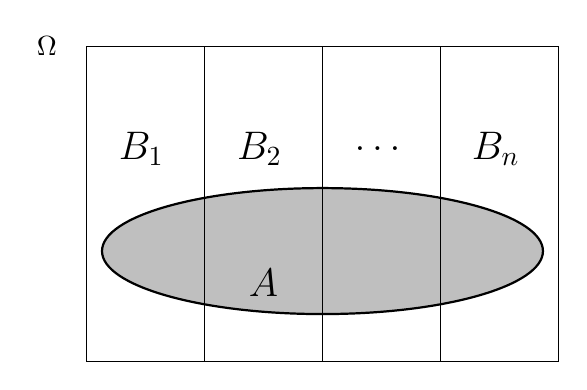
\begin{tikzpicture}
	\draw [fill = white] (-3,-2) -- (-3,2) -- (3,2) -- (3,-2) -- cycle;
	\draw [thick, fill = lightgray] (0,-0.6) ellipse (2.8cm and 0.8cm);
	\draw (1.5,-2) -- (1.5,2);
	\draw (0,-2) -- (0,2);
	\draw (-1.5,-2) -- (-1.5,2);
	%\draw [fill = white] (-0.5,0.8) ellipse (1.6cm and 0.8cm);
	%\draw [thick, fill = white] (0.75,0) circle (1.5);
	%\draw [thick, fill = white] (-0.75,0) circle (1.5);
	%\draw [thick] (0.75,0) circle (1.5);
	\draw (-0.75,-1) node {\Large{$A$}};
	\draw (-3.5,2) node {$\Omega$};
	\draw (-2.3,0.7) node {\Large{$B_1$}};
	\draw (-2.3+1.5,0.7) node {\Large{$B_2$}};
	\draw (-2.3+3,0.7) node {\Large{$\ldots$}};
	\draw (-2.3+4.5,0.7) node {\Large{$B_n$}};
	%\draw (0,0) node {$A \cap B$};
	\end{tikzpicture}
	%\caption{Venn Diagram of $A$ and $A^c.$}
	\end{center}

\noindent

\noindent In the diagram we have drawn another event, $A$, shaded in grey. The law of total probability, which we will now derive, will help us find $P(A)$. Consider the following diagrams

\bigskip
\noindent
\begin{minipage}{.25\textwidth}
	\begin{center}
	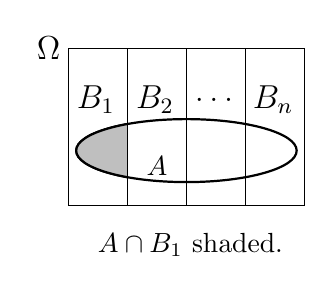
\begin{tikzpicture} [scale = 0.5]
	\draw [fill = white] (-3,-2) -- (-3,2) -- (3,2) -- (3,-2) -- cycle;
	\draw [thick, fill = white] (0,-0.6) ellipse (2.8cm and 0.8cm);
	\scope
	\clip (-1.5,-2) -- (-1.5,2) -- (-3,2) -- (-3,-2) -- cycle;
	\draw [thick, fill = lightgray] (0,-0.6) ellipse (2.8cm and 0.8cm);
	\endscope
	\draw (1.5,-2) -- (1.5,2);
	\draw (0,-2) -- (0,2);
	\draw (-1.5,-2) -- (-1.5,2);
	%\draw [fill = white] (-0.5,0.8) ellipse (1.6cm and 0.8cm);
	%\draw [thick, fill = white] (0.75,0) circle (1.5);
	%\draw [thick, fill = white] (-0.75,0) circle (1.5);
	%\draw [thick] (0.75,0) circle (1.5);
	\draw (-0.75,-1) node {$A$};
	\draw (-3.5,2) node {\large{$\Omega$}};
	\draw (-2.3,0.7) node {\large{$B_1$}};
	\draw (-2.3+1.5,0.7) node {\large{$B_2$}};
	\draw (-2.3+3,0.7) node {\large{$\ldots$}};
	\draw (-2.3+4.5,0.7) node {\large{$B_n$}};
	\draw (0.1,-3) node {$A \cap B_1$ shaded.};
	%\draw (0,0) node {$A \cap B$};
	\end{tikzpicture}
	%\caption{Venn Diagram of $A$ and $A^c.$}
	\end{center}
\end{minipage}% This must go next to `\end{minipage}`
\begin{minipage}{.25\textwidth}
	\begin{center}
	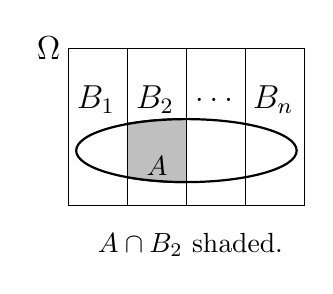
\begin{tikzpicture} [scale = 0.5]
	\draw [fill = white] (-3,-2) -- (-3,2) -- (3,2) -- (3,-2) -- cycle;
	\draw [thick, fill = white] (0,-0.6) ellipse (2.8cm and 0.8cm);
	\scope
	\clip (0,-2) -- (0,2) -- (-1.5,2) -- (-1.5,-2) -- cycle;
	\draw [thick, fill = lightgray] (0,-0.6) ellipse (2.8cm and 0.8cm);
	\endscope
	\draw (1.5,-2) -- (1.5,2);
	\draw (0,-2) -- (0,2);
	\draw (-1.5,-2) -- (-1.5,2);
	%\draw [fill = white] (-0.5,0.8) ellipse (1.6cm and 0.8cm);
	%\draw [thick, fill = white] (0.75,0) circle (1.5);
	%\draw [thick, fill = white] (-0.75,0) circle (1.5);
	%\draw [thick] (0.75,0) circle (1.5);
	\draw (-0.75,-1) node {$A$};
	\draw (-3.5,2) node {\large{$\Omega$}};
	\draw (-2.3,0.7) node {\large{$B_1$}};
	\draw (-2.3+1.5,0.7) node {\large{$B_2$}};
	\draw (-2.3+3,0.7) node {\large{$\ldots$}};
	\draw (-2.3+4.5,0.7) node {\large{$B_n$}};
	\draw (0.1,-3) node {$A \cap B_2$ shaded.};
	%\draw (0,0) node {$A \cap B$};
	\end{tikzpicture}
	%\caption{Venn Diagram of $A$ and $A^c.$}
	\end{center}
\end{minipage}%
\begin{minipage}{.25\textwidth}
	\begin{center}
	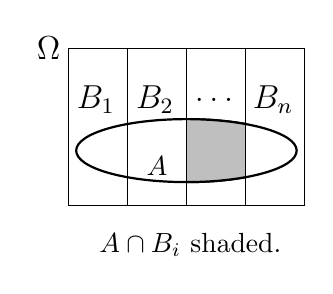
\begin{tikzpicture} [scale = 0.5]
	\draw [fill = white] (-3,-2) -- (-3,2) -- (3,2) -- (3,-2) -- cycle;
	\draw [thick, fill = white] (0,-0.6) ellipse (2.8cm and 0.8cm);
	\scope
	\clip (1.5,-2) -- (1.5,2) -- (0,2) -- (0,-2) -- cycle;
	\draw [thick, fill = lightgray] (0,-0.6) ellipse (2.8cm and 0.8cm);
	\endscope
	\draw (1.5,-2) -- (1.5,2);
	\draw (0,-2) -- (0,2);
	\draw (-1.5,-2) -- (-1.5,2);
	%\draw [fill = white] (-0.5,0.8) ellipse (1.6cm and 0.8cm);
	%\draw [thick, fill = white] (0.75,0) circle (1.5);
	%\draw [thick, fill = white] (-0.75,0) circle (1.5);
	%\draw [thick] (0.75,0) circle (1.5);
	\draw (-0.75,-1) node {$A$};
	\draw (-3.5,2) node {\large{$\Omega$}};
	\draw (-2.3,0.7) node {\large{$B_1$}};
	\draw (-2.3+1.5,0.7) node {\large{$B_2$}};
	\draw (-2.3+3,0.7) node {\large{$\ldots$}};
	\draw (-2.3+4.5,0.7) node {\large{$B_n$}};
	\draw (0.1,-3) node {$A \cap B_i$ shaded.};
	%\draw (0,0) node {$A \cap B$};
	\end{tikzpicture}
	%\caption{Venn Diagram of $A$ and $A^c.$}
	\end{center}
\end{minipage}%
\begin{minipage}{.25\textwidth}
	\begin{center}
	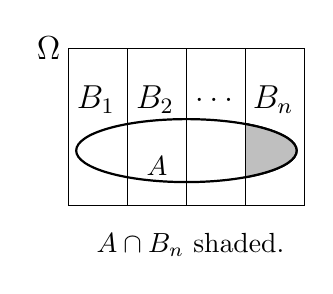
\begin{tikzpicture} [scale = 0.5]
	\draw [fill = white] (-3,-2) -- (-3,2) -- (3,2) -- (3,-2) -- cycle;
	\draw [thick, fill = white] (0,-0.6) ellipse (2.8cm and 0.8cm);
	\scope
	\clip (3,-2) -- (3,2) -- (1.5,2) -- (1.5,-2) -- cycle;
	\draw [thick, fill = lightgray] (0,-0.6) ellipse (2.8cm and 0.8cm);
	\endscope
	\draw (1.5,-2) -- (1.5,2);
	\draw (0,-2) -- (0,2);
	\draw (-1.5,-2) -- (-1.5,2);
	%\draw [fill = white] (-0.5,0.8) ellipse (1.6cm and 0.8cm);
	%\draw [thick, fill = white] (0.75,0) circle (1.5);
	%\draw [thick, fill = white] (-0.75,0) circle (1.5);
	%\draw [thick] (0.75,0) circle (1.5);
	\draw (-0.75,-1) node {$A$};
	\draw (-3.5,2) node {\large{$\Omega$}};
	\draw (-2.3,0.7) node {\large{$B_1$}};
	\draw (-2.3+1.5,0.7) node {\large{$B_2$}};
	\draw (-2.3+3,0.7) node {\large{$\ldots$}};
	\draw (-2.3+4.5,0.7) node {\large{$B_n$}};
	\draw (0.1,-3) node {$A \cap B_n$ shaded.};
	%\draw (0,0) node {$A \cap B$};
	\end{tikzpicture}
	%\caption{Venn Diagram of $A$ and $A^c.$}
	\end{center}
\end{minipage}
\bigskip

\noindent In each diagram, a different section of $A$ is shaded, and $A$ is the union of all of the shaded regions. That is,
\[
A = (A \cap B_1) \cup (A \cap B_2) \cup \ldots \cup (A \cap B_n)
\]
Hence,
\[
P(A) = P\big( (A \cap B_1) \cup (A \cap B_2) \cup \ldots \cup (A \cap B_n) \big)
\]
Since the shaded areas in the diagrams are all mutually disjoint, we know by consequence 1 of the probability measure axioms (see page \pageref{consequence1}), that the probability of the unions is equal to the sum of the probabilities. That is,
\[
P(A) = P(A \cap B_1) + P(A \cap B_2) + \ldots + P(A \cap B_n)
\]
Now, since $P(B_i) > 0$ for all $i$, we know by the multiplication law (section \ref{multiplication law}), that $P(A \cap B_i) = P(A \! \mid \! B_i)P(B_i)$. So, we can rewrite the previous expression as,
\[
P(A) = P(A \! \mid \! B_1)P(B_1) + P(A \! \mid \! B_2)P(B_2) + \ldots + P(A \! \mid \! B_n)P(B_n)
\]
Which is the law of total probabilty. In summation notation it is written as follows: \\

\bigskip
\hfil\fbox{
\begin{minipage}{0.6\columnwidth}{

\vskip 0.02cm
\begin{center}
If there exists an exhaustive family of subsets $B_1,B_2,\ldots,B_n$, where $P(B_i) > 0 $ for all $i$, and $B_i \cap B_j = \varnothing$ for all $i \neq j$. Then for any event $A$,
\[
P(A) = \sum_{i=1}^n P(A\! \mid \! B_i)P(B_i)
\]
\end{center}
}
\end{minipage}}
\bigskip


\subsection{Example} \label{exjockey}
An Egyptian robotics factory has been manufacturing tiny, remote controlled, robotic jockeys to compete in the national pastime of camel racing (no kidding, these robots actually exist, look it up).  The jockeys are tested, and are detected as either `safe' or `unsafe' for use with camels. The probability that they are detected as safe correctly is $0.93$, and the probability that they are detected as unsafe correctly is $0.98$. If in fact $3\%$ are unsafe, then what is the probability that a tested jockey is declared safe? \\

\noindent We define the events that we are interested in to be:
\[
C = \set{\text{A given jockey is tested safe}}, \qquad D = \set{\text{A given jockey actually is safe.}}
\]
The probabilities that we have already been given are
\[
P(D^c) = 0.03, \qquad P(C \! \mid \! D) = 0.93, \qquad P(C^c \! \mid \! D^c) = 0.98.
\]
From these we can use consequence 2 of the probability measure axioms to get
\[
P(D) = 1 - P(D^c) = 0.97, \qquad P(C \! \mid \! D^c) = 1 - P(C^c \! \mid \! D^c) = 0.02.
\]
Now, since $D \cup D^c = \Omega$, and $D \cap D^c = \varnothing$, and since $P(D) > 0$, and $P(D^c) > 0$, we can use the law of total probability to find $P(C)$, 
\begin{align*}
P(C)  & = P(C \! \mid \! D)P(D) + P(C \! \mid \! D^c)P(D^c) \\
	& = 0.93\times 0.97 + 0.02 \times 0.03 \\
	& = 0.9027.
\end{align*}
So the probability that a given jockey is declared safe is $0.9027.$ \\

\noindent Note that we can extend this idea to any diagnostic testing situation where we can have ``false positives'' and ``false negatives.''

\subsection{Bayes' rule} \label{bayes rule}
We consider almost exactly the same situation as we did for the law of total probability. \\

\noindent We have a collection of events $B_1,B_2,\ldots,B_n$, with $\Omega = B_1 \cup B_2 \cup \ldots \cup B_n$, where $P(B_i) > 0$ for all $i$ and $B_i \cap B_j = \varnothing$ for $i \neq j$. There is also another event, $A$, and we assume that we know $P(A)$. The only difference between this scenario and the one for the law of total probability is that now we know $P(A).$ \\

\noindent We want to find the conditional probability of one of the events $B_j$, for some $j \leq n$. That is, we want to find $P(B_j \! \mid \! A)$. In doing so, we will derive Bayes' rule. \\

\noindent Starting with the definition of conditional probability, we have
\[
P(B_j \! \mid \! A)  = \frac{P(B_j \cap A)}{P(A)}
\]
But by the commutative law (see page \pageref{commutative law}) we know $B_j \cap A = A \cap B_j$. So, $P(B_j \cap A) = P(A \cap B_j)$. Now, by the multiplication law we know that $P(A \cap B_j) = P(A \! \mid \! B_j)P(B_j)$. Thus we can write
\[
P(B_j \! \mid \! A) = \frac{P(A \! \mid \! B_j)P(B_j)}{P(A)}.
\]
In the denominator we have $P(A)$. We can use the law of total probability to express $P(A)$ as
\[
P(A) = \sum_{i = 1}^nP(A \! \mid \! B_i)P(B_i).
\]
Substituting this in place of $P(A)$ in the denominator gives Bayes'~rule,
\[
P(B_j \! \mid \! A) = \frac{P(A \! \mid \! B_j)P(B_j)}{\displaystyle{\sum_{i = 1}^nP(A \! \mid \! B_i)P(B_i)}}
\]
\bigskip
\hfil\fbox{
\begin{minipage}{0.6\columnwidth}{

\vskip 0.02cm
\begin{center}
If there exists a family of subsets $B_1,B_2,\ldots,B_n$, where $P(B_i) > 0 $ for all $i$, and $B_i \cap B_j = \varnothing$ for all $i \neq j$. Then for any events, $A$ and $B_j$, where $j \leq n$,
\[
P(B_j \! \mid \! A) = \frac{P(A \! \mid \! B_j)P(B_j)}{\displaystyle{\sum_{i = 1}^nP(A \! \mid \! B_i)P(B_i)}}
\]
\end{center}
}
\end{minipage}}
\bigskip

\noindent Bayes' rule is very important in the correct interpretation of diagnostic tests (see the next example). It is also key in the ``Bayesian'' approach to statistics.
%NEED TO MENTION WHERE BAYESIAN STATISTICS IS INTRODUCED.

%MAY BE A GOOD IDEA TO INTRODUCE CONDITIONAL PROBABILITY TREE DIAGRAMS HERE

\subsection{Example}
What is the probability that a jockey from example \ref{exjockey} is actually unsafe when it has been decared safe?

\noindent Using the events $C$ and $D$ as defined in the previous example, we are looking for the probability $P(D^c \! \mid \! C)$, i.e., the probability that a jockey is actually unsafe, $D^c$, given that it is tested safe, $C.$ \\

\noindent Applying Bayes' rule we get
\[
P(D^c \! \mid \! C) = \frac{P(C \! \mid \! D^c)P(D^c)}{P(C \! \mid \! D^c)P(D^c) + P(C \! \mid \! D)P(D)}
\]
We found (or were given) all of the required values in example \ref{exjockey}. Substituting in these values gives,
\[
P(C^c \! \mid \! D) = \frac{0.02\times0.03}{0.02\times 0.03 + 0.93 \times 0.97} \approx 0.0007.
\]
So the probability that a jockey is dangerous when it has been declared safe is approximately 0.0007, i.e., roughly 7 in every 10,000 jockeys.
